\section{Results}
\label{sec:results}

The number of operations in the compression algorithm with respect to the number of stored incremental or time steps (the number of rows in the matrix $\mtrx{A}$) is depicted in Figure \ref{fig:ExeTime_rows} while the number of operations with respect to the number of points, where the results are stored (the number of columns of the matrix $\mtrx{A}$), is depicted in Figure \ref{fig:ExeTime_columns}. Especially on Figure \ref{fig:ExeTime_columns} is clearly visible that the randomized SVD algorithm is much faster than the classical one.

These results confirm that the SVD implementation has computational complexity $O(m^2n)$, where $m$ is number of rows, $n$ is number of columns, and $m < n$. In case of $m > n$ the complexity would be $O(mn^2)$ as the algorithm takes advantage of non-squareness in that its complexity is only linear in the greater dimension.

\begin{figure}[H]
\centering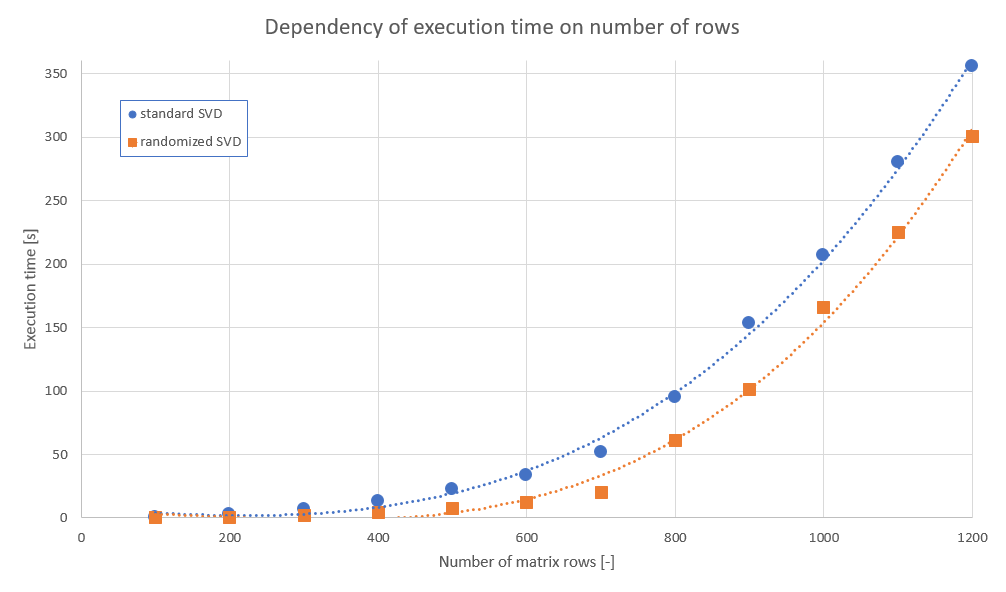
\includegraphics[width=\textwidth]{figures/executionTime_varyingRows}
\caption{Dependency of SVD execution time on number of rows of an input matrix (having fixed number of columns).}
\label{fig:ExeTime_rows}
\end{figure}

\begin{figure}[H]
\centering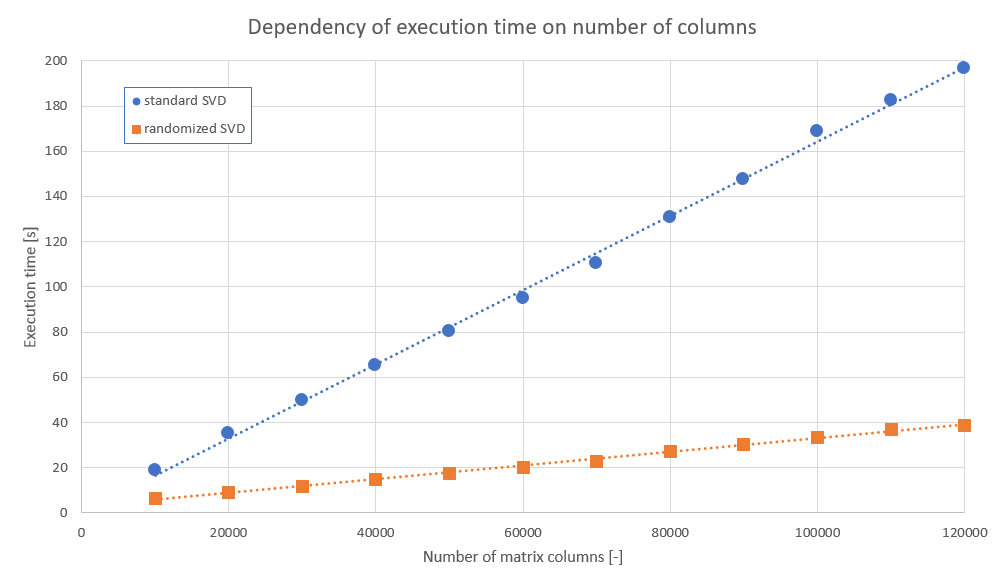
\includegraphics[width=\textwidth]{figures/executionTime_varyingColumns}
\caption{Dependency of SVD execution time on number of columns of an input matrix (having fixed number of rows).}
\label{fig:ExeTime_columns}
\end{figure}

% reactor containment
Behavior of the compression strategy introduced is presented on three real world examples. First example is an analysis of aging of nuclear power plant's containment made from prestressed concrete. Finite element mesh used in this analysis is in Figure \ref{fig:temelin:mesh}. More details about the analysis can be found in \cite{Kruis2012} and \cite{Koudelka2009}. This analysis includes high number of analysis time steps (thousands) with very little differences between them. There is therefore potential for compression ratio to be very high as proven in Figure \ref{fig:temelin:NRMSD} that examines the impact of changes in the compression ratio to the mean error of approximation.

\begin{figure}[H]
\centering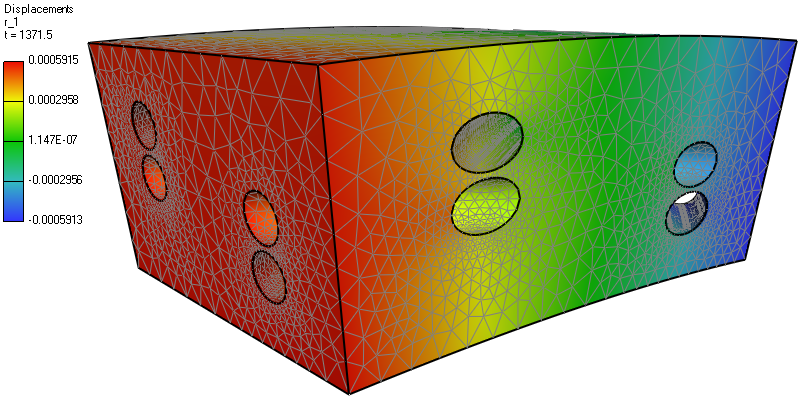
\includegraphics[width=\textwidth]{figures/temelin_screenshot}
\caption{Segment of containment analyzed. Results visualization (displacement field, x component).}
\label{fig:temelin:mesh}
\end{figure}

\begin{figure}[H]
\centering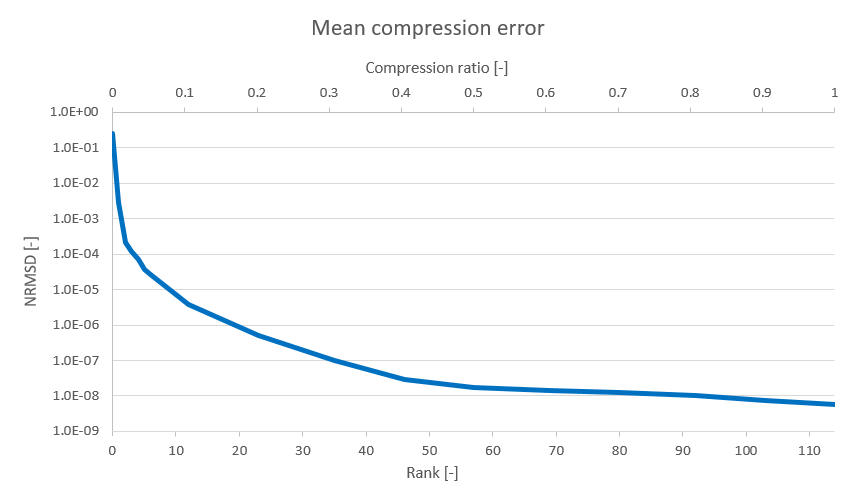
\includegraphics[width=\textwidth]{figures/temelin_NRMSD}
\caption{Dependence of Normalized Rooted Mean Squared Deviation on Compression ratio for reactor containment analysis results.}
\label{fig:temelin:NRMSD}
\end{figure}

% geological layers
Figure \ref{fig:chotkova:mesh}  shows results from an analysis of geological layers which was based on theory plasticity. More details can be found in \cite{Koudelka2006}. This project was chosen mainly to study behavior of compression algorithm when dealing with high discontinuities in data in spatial dimension (as can be seen in visualization). As summarized in Figure \ref{fig:chotkova:NRMSD} and Figure \ref{fig:chotkova:MaxError} this has negligible effect on quality of compression.

\begin{figure}[H]
\centering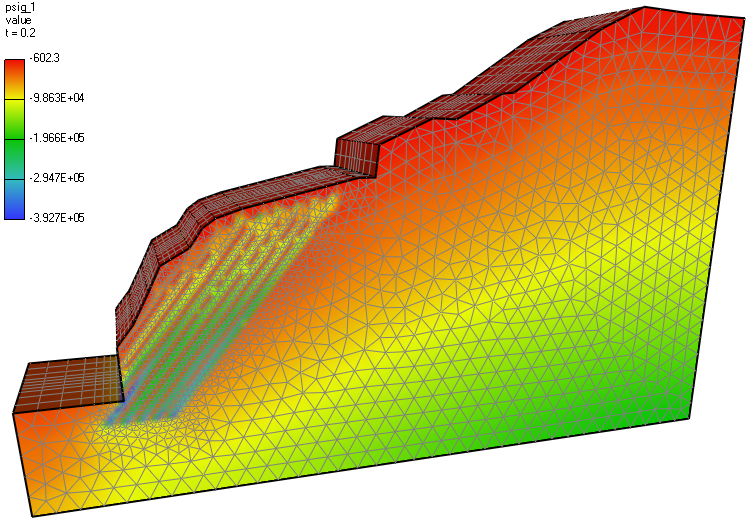
\includegraphics[width=\textwidth]{figures/chotkova_screenshot}
\caption{Analysis of geological layers. Results visualization (stress field, sigma XX component).}
\label{fig:chotkova:mesh}
\end{figure}

\begin{figure}[H]
\centering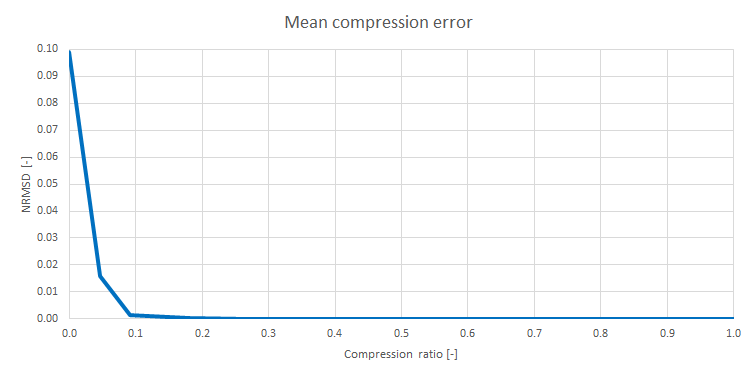
\includegraphics[width=\textwidth]{figures/chotkova_NRMSD}
\caption{Dependence of Normalized Rooted Mean Squared Deviation on Compression ratio for results of geological layers project.}
\label{fig:chotkova:NRMSD}
\end{figure}

\begin{figure}[H]
\centering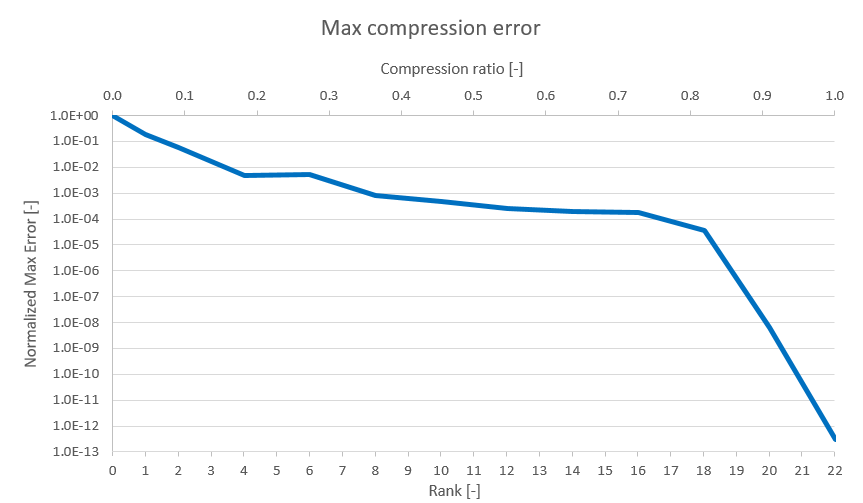
\includegraphics[width=\textwidth]{figures/chotkova_MaxError}
\caption{Dependence of Normalized Maximum Error on Compression ratio for results of geological layers project.}
\label{fig:chotkova:MaxError}
\end{figure}

% reactor vessel 2D
Figure \ref{fig:mechaxisym:mesh} contains visualization of results of two-dimensional analysis, where axisymmetric description was used for analysis of aging of a reactor vessel. Details about the analysis can be found in \cite{Kruis2005}. There are exactly 232 analysis time steps. The resulting data has linear function character with several discontinuities in temporal dimension. There are few time steps in which resulting discrete functions have very different values compared to neighboring time steps. This was supposed to have negative impact on the quality of compression. However, as can be seen in Figure \ref{fig:mechaxisym:NRMSD}, the quality is better than expected; e.g., if the rank of approximation matrix is set to 3 (compared to 232 being the rank of the original matrix) the normalized relative error ($\mathit{NRMSD}$) does not exceed $10^{-5}$.

\begin{figure}[H]
\centering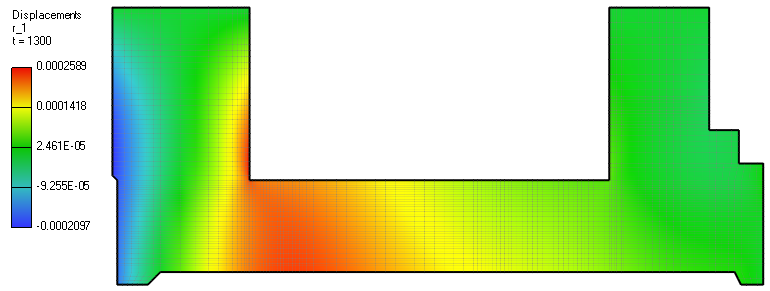
\includegraphics[width=\textwidth]{figures/mechaxisym_screenshot}
\caption{2D model of a reactor vessel. Results visualization (displacement field, x component).}
\label{fig:mechaxisym:mesh}
\end{figure}

\begin{figure}[H]
\centering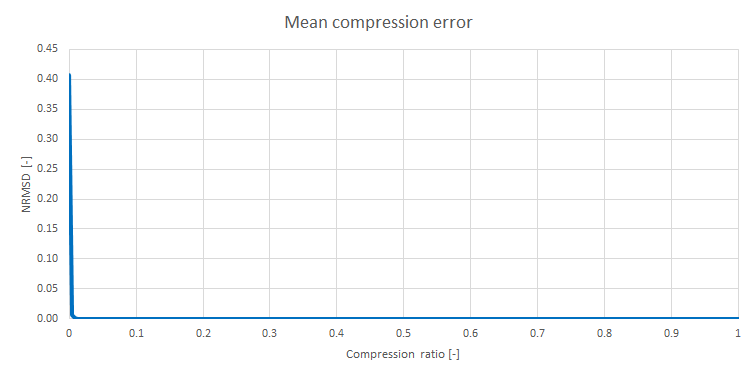
\includegraphics[width=\textwidth]{figures/mechaxisym_NRMSD}
\caption{Dependence of Normalized Rooted Mean Squared Deviation on Compression ratio for reactor vessel analysis results.}
\label{fig:mechaxisym:NRMSD}
\end{figure}

% PSNR
Figure \ref{fig:PSNR} summarizes the compression error for all three benchmarks using logarithmic scale to make the differences more visible. Peek signal to noise ratio ($\mathit{PSNR}$) metric is used (see Equation \ref{eq:psnr-def} for definition). Figure \ref{fig:PSNR_rand} contains the same comparison for the randomized SVD algorithm.

\begin{figure}[H]
\centering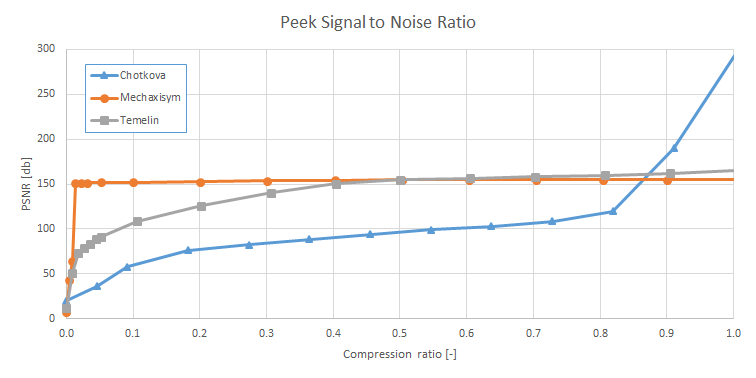
\includegraphics[width=\textwidth]{figures/PSNR}
\caption{Comparison of Peek signal to noise ratio value calculated for different decompositions.}
\label{fig:PSNR}
\end{figure}

\begin{figure}[H]
\centering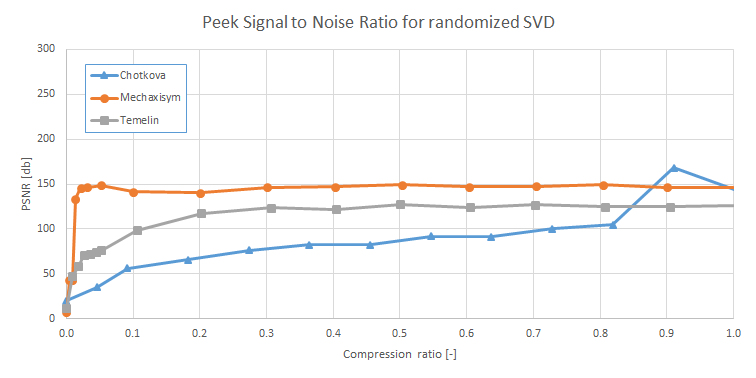
\includegraphics[width=\textwidth]{figures/PSNR_rand}
\caption{Comparison of Peek signal to noise ratio value for different randomized decompositions.}
\label{fig:PSNR_rand}
\end{figure}

% Execution times
Besides the error also the execution speed of compression algorithm was measured. In Figure \ref{fig:temelin:ExeTime} is comparison of execution times for standard versus randomized SVD compression algorithms. Interestingly, execution time of standard SVD is independent of target rank whereas execution time of randomized SVD decreases linearly with decreasing target rank. If the rank is known ahead of time the fact can be taken advantage of.

\begin{figure}[H]
\centering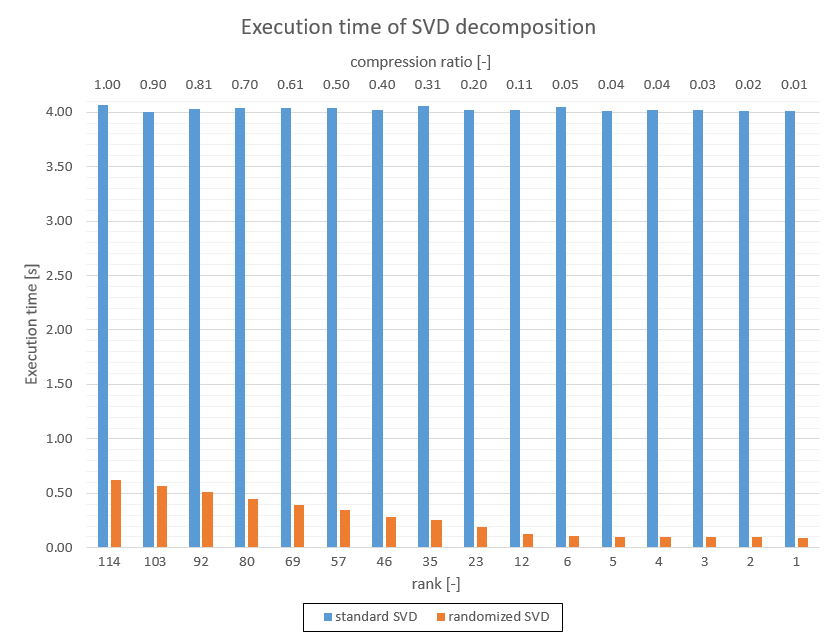
\includegraphics[width=\textwidth]{figures/temelin_ExecutionTime}
\caption{Variation of execution time of standard and randomized decompositions calculated for reactor containment analysis results.}
\label{fig:temelin:ExeTime}
\end{figure}

The memory consumption of compressed results for reactor containment analysis is summarized in Table \ref{tab:mem-consum}. For different values of compression ratio shows memory size in megabytes. Compression ratio $c$ is an input parameter to the compression algorithm specifying amount of singular values ought to be removed from the SVD decomposition as follows from the equation (\ref{eq:rank-from-comp-ratio}). Size factor describes the final outcome of compression when compared to the original size.

\begin{table}[H]
\centering
    \begin{tabular}{| r | r | r |}
    \hline
    compression ratio ($c$) & memory consumption [MB] & size factor \\ \hline \hline
    1.00 & 2002.1 & 1 \\ \hline
    0.50 & 1006.9 & 0.5002 \\ \hline
    0.10& 211.9 & 0.1053 \\ \hline
    0.01 & 35.3 & 0.0176 \\ \hline
    \end{tabular}
    \caption{Memory consumption of compressed results. 3D reactor containment analysis.}
	\label{tab:mem-consum}
\end{table}
